\section{Modelling of Bayesian Network}
\begin{frame}{Simplification of Bayesian Network}
    In this paper, the resource node is introduced to simplify the Bayesian network, the following figure shows two Bayesian network with/without resource node.
    \begin{figure}
      \centering
      \resizebox{\textwidth}{!}{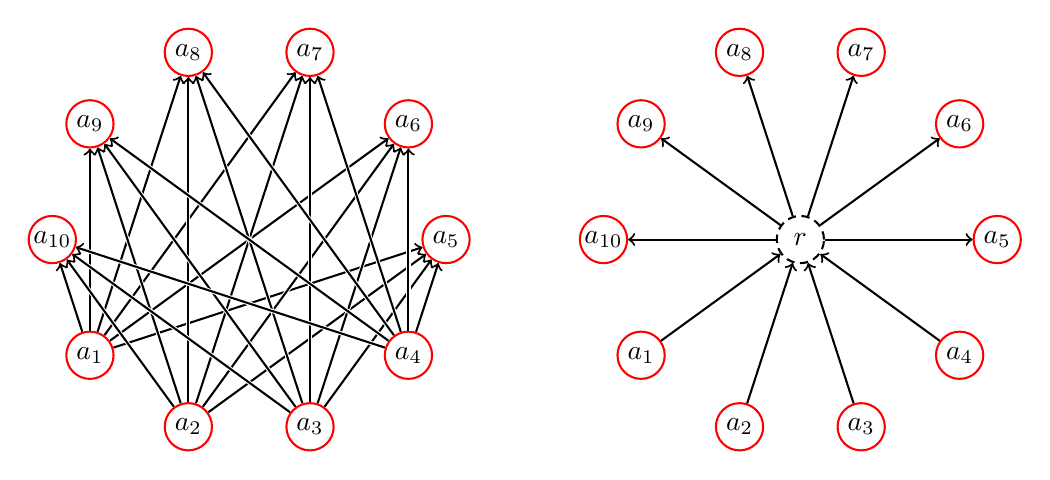
\begin{tikzpicture}[line width = 0.75pt,
                    basic/.style    = {circle, minimum size = 0.6cm, inner sep = 0pt, align = center},
                    attack/.style   = {draw = red,   basic},
                    resource/.style = {draw, densely dashed, basic},
                    function/.style = {draw = blue,  basic},
                    incident/.style = {draw = green, basic},
                    asset/.style    = {draw = black, basic}
                    ]
    \linespread{1}
    \uncover<2->{
    \foreach \i in {1, 2, ..., 10}
        \path (0,0) ++ (180 + 36*\i:2.5cm) node[attack] (aa\i) {$a_{\i}$};

    \foreach \i in {1, 2, 3, 4}{
        \foreach \j in {5, 6, ..., 10}{
            \draw[line width = 1.5pt, white] (aa\i) -- (aa\j);
            \draw[->] (aa\i) -- (aa\j);
        }
    }
    }
    
    \uncover<3>{
    \node[resource] (r) at (7, 0) {$r$};
    \foreach \i in {1, 2, ..., 10}
        \path (r) ++ (180 + 36*\i:2.5cm) node[attack] (a\i) {$a_{\i}$};

    \foreach \i in {1, 2, 3, 4}{
        \draw[->] (a\i) -- (r);
    }

    \foreach \i in {5, 6, ..., 10}{
        \draw[->] (r) -- (a\i);
    }
    }


    
\end{tikzpicture} }
    \end{figure}
\end{frame}

\begin{frame}{Estimation of Fuzzy Conditional Probabilities}
    In this paper, there are only two states of a node in the Bayesian network, which is shown as follows.
    \[
    x = \left\{
        \begin{array}{ll}
            F, & \text{the corresponding event of node $x$ does not happen,} \\
            T, & \text{the corresponding event of node $x$ does happen.}
        \end{array}
    \right.
    \]

    \pause
    Assume that a node $x$ has $m$ parent nodes $\pnode{x}_1, \pnode{x}_2, \cdots, \pnode{x}_m$. There exists a conditional probability table of the node $x$, which is shown as follows.

    \extrarowsep = -1pt
    \begin{tabu}to \textwidth{X[-1, l, $]|*6{X[c, $]}}
        \pnode{x}_1     & F      & F      & \cdots & T         & T         & T       \\
        \pnode{x}_2     & F      & F      & \cdots & T         & T         & T       \\
        \hspace{5pt}\vdots   & \vdots & \vdots & \ddots & \vdots    & \vdots    & \vdots  \\
        \pnode{x}_{m-2} & F      & F      & \cdots & T         & T         & T       \\
        \pnode{x}_{m-1} & F      & F      & \cdots & F         & T         & T       \\
        \pnode{x}_{m}   & F      & T      & \cdots & T         & F         & T       \\
        \tabucline{-}
        \hspace{3pt}x   & p_1    & p_2    & \cdots & p_{2^m-2} & p_{2^m-1} & p_{2^m} \\
    \end{tabu}
\end{frame}

\begin{frame}{Estimation of Fuzzy Conditional Probabilities}
    Because the size of historical data of malicious attacks for ICSs is too small, the conditional probabilities from the statistical analysis of historical data is not always accurate. To solve this problem, in this paper, the fuzzy probability is used to replace the crisp probability which is hard to be obtained.

    \pause
    This fuzzy probability is denoted by $\fp{p} = \fpe{}$, where $0 \leq \pl{p} \leq p \leq \pu{p} \leq 1$. The following figure shows the fuzzy number $\fp{p}$.
    \begin{figure}
      \centering
      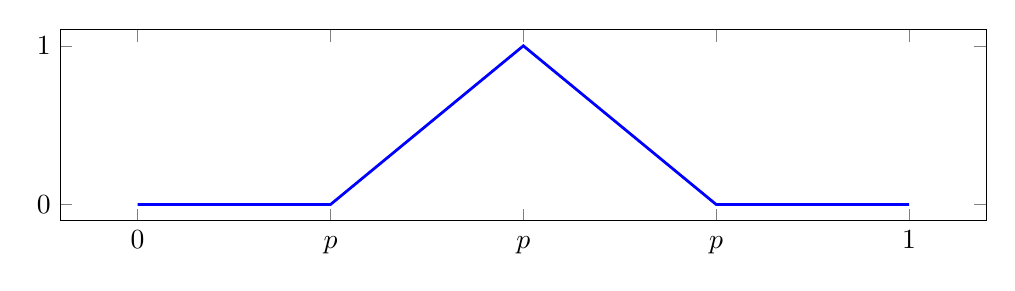
\begin{tikzpicture}
    \linespread{1}
    \begin{axis}[
        width            = 1.1\textwidth,
        height           = 4cm,
        xtick            = {0,        1,   2,        3, 4},
        xticklabels      = {0, $\pl{p}$, $p$, $\pu{p}$, 1},
        xticklabel style = {text height = 1.5ex},
        ytick            = {0, 1},
        yticklabels      = {0, 1}]

        \addplot[
            line width   = 1pt,
            mark         = none,
            draw         = blue]
            coordinates {
                (0,0)
                (1,0)
                (2,1)
                (3,0)
                (4,0)
            };
    \end{axis}
\end{tikzpicture} 
    \end{figure}
    \vspace{-20pt}
\end{frame}

\begin{frame}{Estimation of Fuzzy Conditional Probabilities}
    Two strategies to obtain the fuzzy conditional probabilities:\pause
    \begin{itemize}
      \item If the number of fuzzy conditional probabilities is not very large, the experts can estimate the fuzzy conditional probabilities case-by-case.\pause
      \item If there are a mount of fuzzy conditional probabilities to be estimated, a group of fuzzy probabilities are suggested to be established in advance.
    \end{itemize}
    \vspace{5pt}\pause
    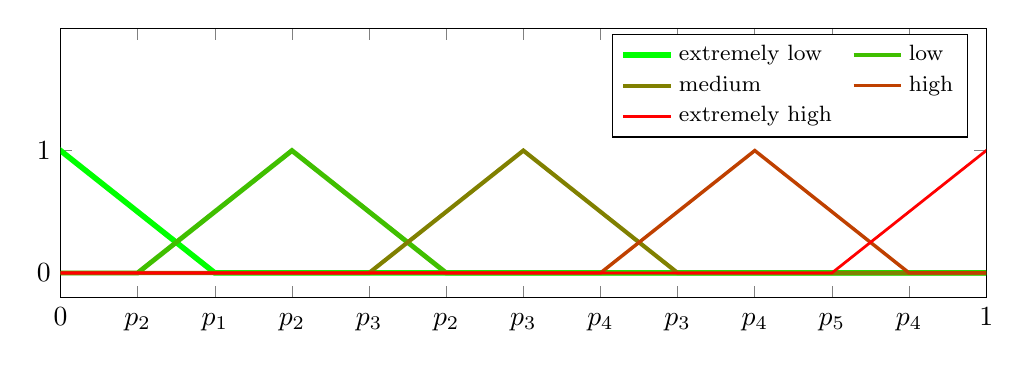
\begin{tikzpicture}
    \linespread{1}

    \pgfmathsetmacro\fuzzywidth{1.3333}

    \begin{axis}[
        width            = 1.1\textwidth,
        height           = 5cm,
        legend columns   = 2,
        legend style     = {legend cell align = left, font = \footnotesize, /tikz/column 2/.style={column sep=5pt}},
        xtick            = {0, 0.33333, ..., 4},
        xticklabels      = {$0$, $\pl{p}_2$, $\pu{p}_1$, $p_2$, $\pl{p}_3$, $\pu{p}_2$, $p_3$, $\pl{p}_4$, $\pu{p}_3$, $p_4$, $\pl{p}_5$, $\pu{p}_4$, 1},
        xticklabel style = {text height = 1.5ex},
        xmin             = 0,
        xmax             = 4,
        ytick            = {0, 1},
        yticklabels      = {$0$, $1$},
        ymax             = 2]

        \pgfplotsinvokeforeach{0,25,...,100}{
        \addplot[draw = red!#1!green, line width = 2pt-#1*0.01pt]
            coordinates {
                (-1, 0)
                (0.04*#1 - 0.5*\fuzzywidth, 0)
                (0.04*#1, 1)
                (0.04*#1 + 0.5*\fuzzywidth, 0)
                (6, 0)
            };
        }

        \legend{extremely low, low, medium, high, extremely high}
        \end{axis}
\end{tikzpicture} 
    \vspace{-10pt}
\end{frame} 